\chapter{\ch{Cr4Fe4Mn4Ni4Si32}}
\label{appendix:equi}

\section{Density of states}

\begin{figure}[H]
	\centering
	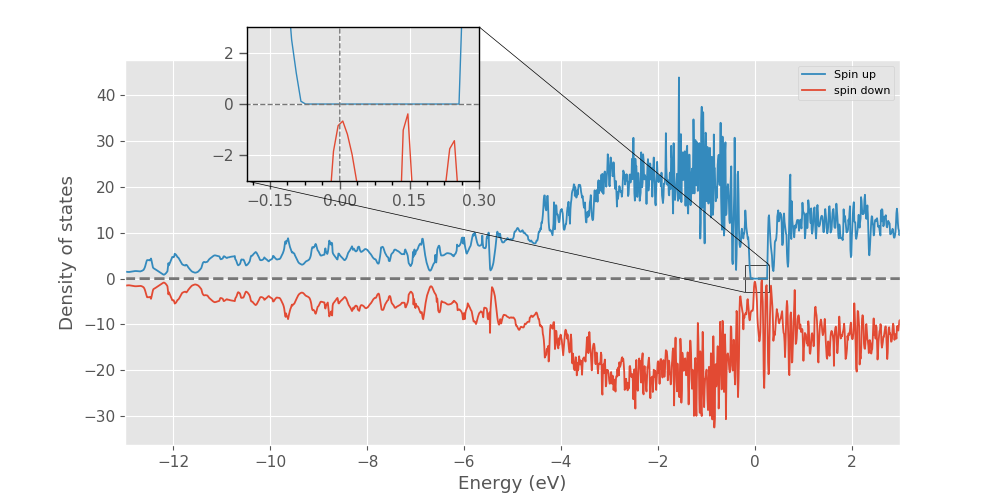
\includegraphics[width=\textwidth]{results/fesi2/A_TDOS.png}
	\caption{Density of states SQS A \ch{(CrFeMnNi)Si2} with PBE.}
\end{figure}

\begin{figure}[H]
	\centering
	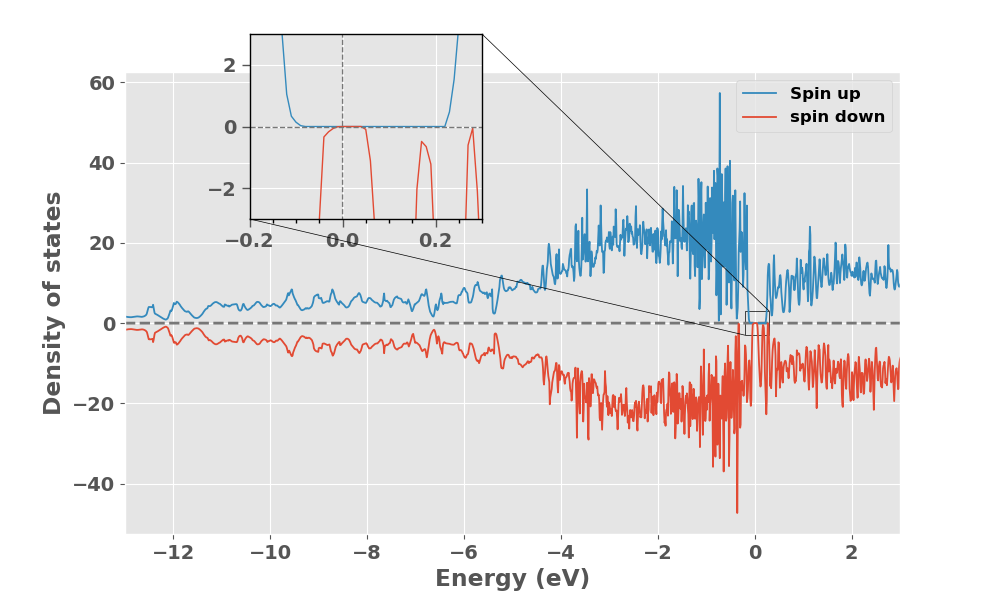
\includegraphics[width=\textwidth]{results/fesi2/E_TDOS.png}
	\caption{Density of states SQS E \ch{(CrFeMnNi)Si2} with PBE.}
\end{figure}

\begin{figure}[H]
	\centering
	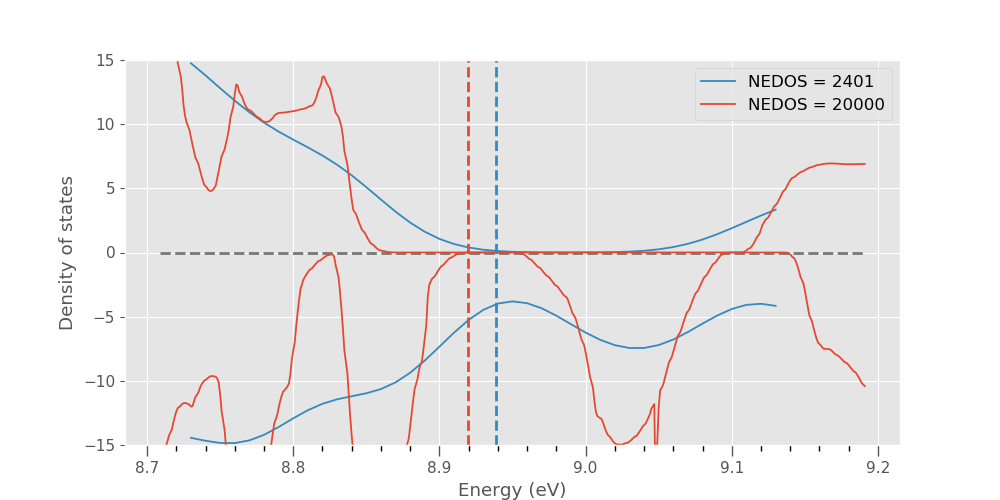
\includegraphics[width=\textwidth]{results/fesi2/C_DOS.png}
	\caption{Density of states SQS C \ch{(CrFeMnNi)Si2} with PBE. Nedos represent the number of points in the DOS calculation.}
\end{figure}


\section{Projected density of states}

\begin{figure}[H]
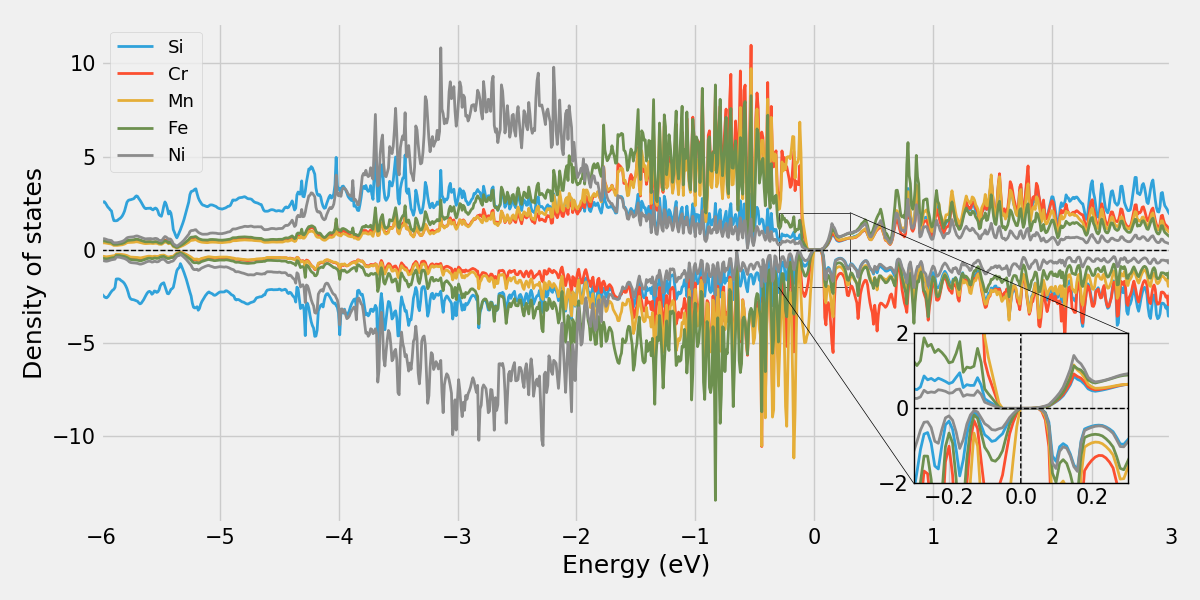
\includegraphics[width=\textwidth]{results/fesi2/A_PDOS.png}
\caption{Projected density of states SQS A}
\end{figure}

\begin{figure}[H]
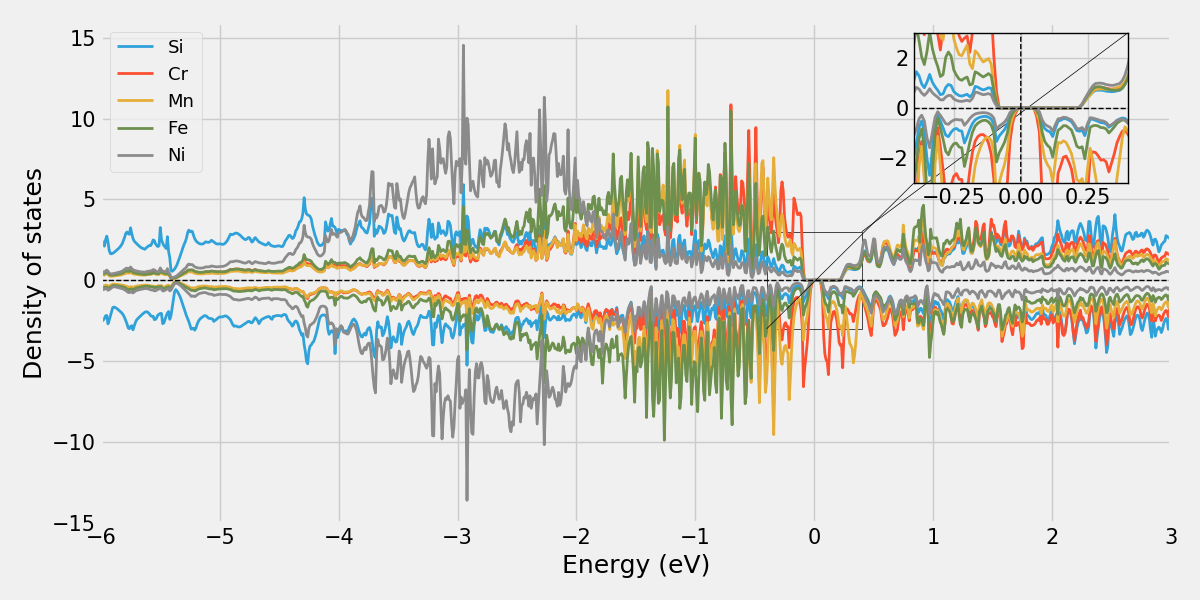
\includegraphics[width=\textwidth]{results/fesi2/B_PDOS.png}
\caption{Projected density of states SQS B}
\end{figure}

\begin{figure}[H]
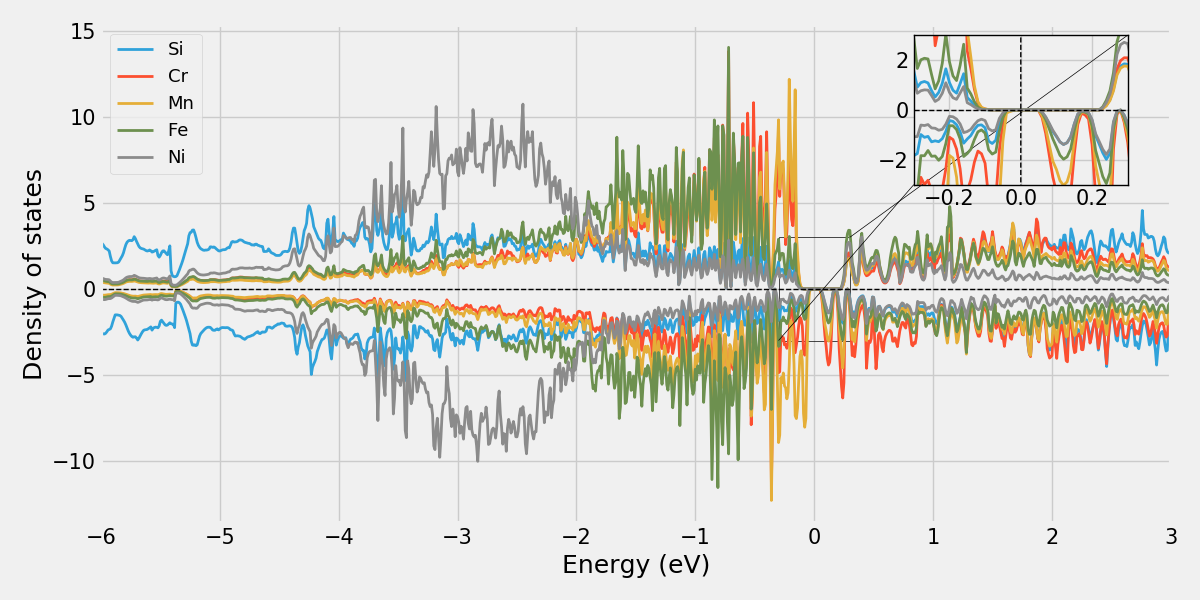
\includegraphics[width=\textwidth]{results/fesi2/E_PDOS.png}
\caption{Projected density of states SQS E}
\end{figure}

\section{Charge density}

\begin{figure}[H]
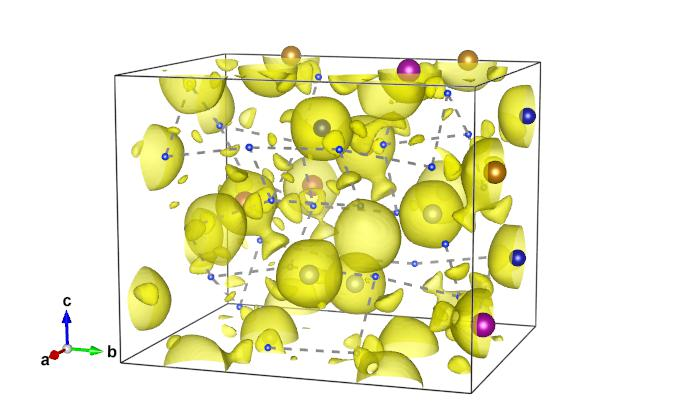
\includegraphics[width=\textwidth]{results/fesi2/C_CHGCAR.jpg}
\caption{Charge density of SQS C.}
\end{figure}
